\documentclass[a4paper]{IEEEtran}

% Ein paar hilfreiche Pakete
\usepackage[utf8]{inputenc}
\usepackage[ngerman]{babel}
\usepackage{graphicx}
\usepackage{amsmath}
\usepackage{amssymb}
\usepackage{mathtools}
\usepackage{subcaption}
\usepackage{hyperref}

\mathtoolsset{showonlyrefs}

\markboth{Proseminar WS 16/17: Anthropomatik: Von der Theorie zur Anwendung}{Proseminar SS 16: Anthropomatik: Von der Theorie zur Anwendung}

% Hier den Titel des eigenen Proseminars eitnragen
\title{Discovery of Processes}

% Hier deinen eigenen Namen
\author{Maximilian Franz}


\begin{document}
\maketitle

% Zusammenfassung
\begin{abstract}
TODO
\end{abstract}

% Erster Abschnitt
\section{Introduction}
Some intro text

\section{Ein paar Hinweise}

Vor eine Subsection gehören immer noch ein paar einleitende Worte!

\subsection{Absätze, etc.}

Ein neuer Absatz sollte nicht durch einen Zeilenumbruchs-Befehl, sondern durch eine Leerzeile im Code erzeugt werden.

Das hier ist richtig.
\\ Das hier nicht.

\subsection{Formeln}

So können Formeln gesetzt und referenziert werden:
\begin{equation}
    a = b + c \,.
    \label{eq:name}
\end{equation}
Laut \eqref{eq:name} ist $a=b+c$. Formeln sind Teil des Fließtextes und sollten deshalb korrekt mit Punkten und Kommata interpunktiert werden.  Das \texttt{\textbackslash,} fügt dabei einen kleinen Abstand zwischen Formel und Interpunktion ein.

Mehrzeiliger Formelsatz mit der \emph{split} Umgebung innerhalb der \emph{equation} Umgebung:
\begin{equation}
    \begin{split}
        a      &= b + c \,, \\
        a_{ij} &= b_{ij} + c_{ij} \,.
    \end{split}
\end{equation}

Funktionen sollen in Formeln \emph{nicht} mit mathematischer Schrift gesetzt werden.
Dazu gibt es in LaTeX für fast alle Funktionen schon Makros, z.B. 
\begin{align}
    y = \sin(x)\,,
\end{align}
nicht 
\begin{align}
    y = sin(x)
\end{align}
benutzen. Für nicht vorhandene Funktionen kann \emph{operatorname} eingesetzt werden:
\begin{equation}
    y = \operatorname{spur}(X) \,.
\end{equation}

\subsection{Bilder}

So werden Bilder eingebunden (als pdf, jpg oder png):

\begin{figure}[!h]
    \centering
    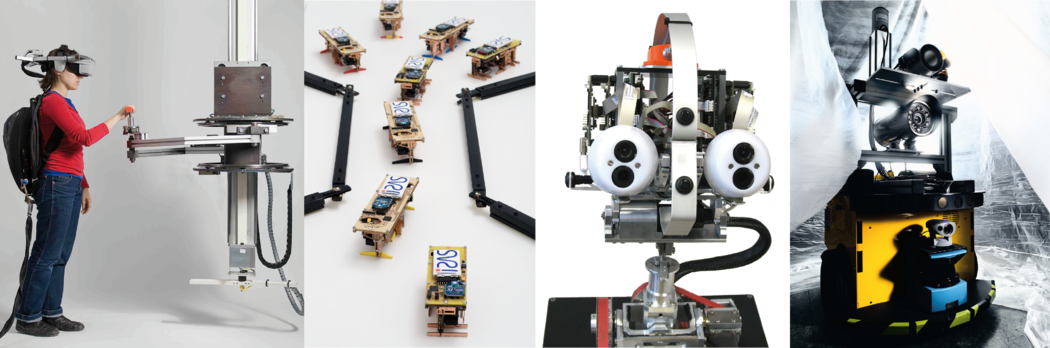
\includegraphics[width=0.48\textwidth]{Bild.png}
    \caption{Hier kommen weitere Erklärungen zum Bild.}
    \label{fig:bild}
\end{figure}

Auf diese Abbildung wird dann mit Abb. \ref{fig:bild} verwiesen.

\subsection{Zitate}

Immer korrekt zitieren \cite{yaakov_bar-shalom_estimation_2001}!

\subsection{LaTeX Hilfe}

Diese Website ist sehr nützlich:

\url{http://en.wikibooks.org/wiki/LaTeX}

\section{Zusammenfassung und Ausblick}

In dieser Ausarbeitung wurde ...

% Literaturverzeichnis in Literatur.bib
% (z.B. per Hand oder mit Zotero, Jabref, etc. editieren) 
\bibliographystyle{ieeetr}
\bibliography{references}
\end{document}
